\chapter{Návrh analýzy}
\label{possible-analysis-strategies}

V tejto kapitole popisujem návrh na vypracovanie analýzy nasadenia a využívania technológie NEL.

\subsubsection{Cieľ a rozsah}

Cieľom práce je analyzovať nasadenie technológie NEL na webe. 
Vďaka dostupným zdrojom dát popisovaných v kapitole \ref{data-sources-available-for-research} je možné skúmať stav využívania NEL:
\begin{enumerate}
    \item v histórií prehliadania webu zaznamenanej v dátach poskytovaných projektom HTTP Archive,
    \item v súčasnosti, použitím automatizovaného webového prehliadania.
\end{enumerate}

Na základe konzultácie s vedúcim tejto práce, pánom Polčákom, som sa rozhodol analýzu zhotoviť pre čo 
najrozsiahlejšie obdobie.
Zámerom je pokúsiť sa pokryť celé obdobie, za ktoré sa NEL doteraz používalo, no závisí na zdrojoch použitých pre analýzu, či budú všetky potrebné dáta dostupné.
Ako počiatočný dátum môžem zvoliť 25. september 2018, kedy autori tejto technológie publikovali jej špecifikáciu (viď sekciu \ref{network-error-logging}).
Od tohto počiatočného dátumu chcem zhotoviť prieskum až po mesiac pred odovzdaním tejto práce -- apríl 2024.

\subsubsection{Existujúca analýza}

Taktiež som sa v rámci konzultácií zameral na získanie cenných informácií a poučení z už existujúcej analýzy z roku 2023,
ktorú zhotovil pán Polčák spolu s jeho kolegom, pánom Jeřábkom \cite{nel-http-archive}.
Je zameraná na získanie metrík ako celkové využívanie NEL na množine skúmaných domén (viď obrázok \ref{fig:polcak-analysis}), aké NEL kolektory dané domény používajú a v akých konfiguráciách sa nasadené NEL vyskytuje.
Časové obdobie, za ktoré bola analýza zhotovená, tvorili februárové mesiace každého roku od 2018 do 2023. 
Za toto obdobie sa im podarilo zistiť, že počiatočné využitie NEL bolo 0\% a do februára roku 2023 stúplo na 11.73\% skúmaných domén.
Toto percento predstavuje z celkového počtu skúmaných domén 2 247 233 jedinečných domén.

\begin{figure}[!htb]
\begin{center}
    % 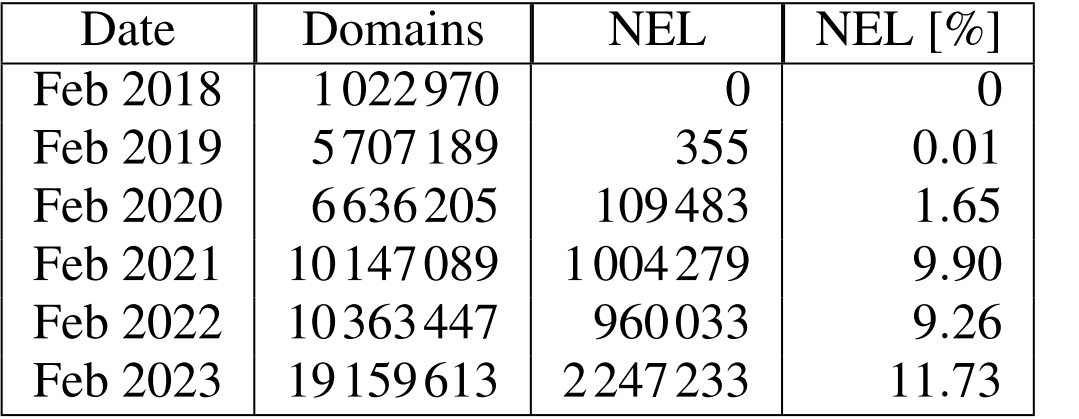
\includegraphics[width=0.5\linewidth]{obrazky-figures/polcak-analysis.png}
    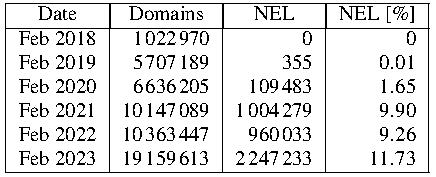
\includegraphics[width=0.55\linewidth]{obrazky-figures/polcak-analysis-hd.pdf}
    \caption{Využitie NEL na skúmaných doménach v analýze vypracovanej vo vedeckom článku Ing. Libora Polčáka Ph.D. a Ing. Kamila Jeřábka. Obrázok tabuľky prevzatý z \cite{nel-http-archive}.}
    \label{fig:polcak-analysis}
\end{center}
\end{figure}

\pagebreak

Zistil som, že ako zdroj dát bol použitý HTTP Archive, ktorým sa zaoberá aj moja práca.
Je však dôležité poznamenať, že predošlá analýza bola vypracovaná iba za pomoci využitia 
práve jedného zdroja dostupného na každej skúmanej doméne \cite{nel-http-archive}.
Tým pádom neboli dostupné dáta využité naplno a ostal priestor pre vylepšenia.

\subsubsection{Prieskum možností pre vylepšenia}

Preskúmal som spôsob, ktorý vo vyššie uvedenej práci použili na získavanie HTTP Archive dát.
Bol použitý nástroj pre sťahovanie dát z Google Cloud BigQuery, ktorý naprogramoval pán 
Jeřábek\footnote{\url{https://github.com/kjerabek/nel-http-archive-analysis}}.
Počas testovania tohto nástroja som zistil, že je možné vylepšiť ho tak, aby som odstránil predošlú limitáciu.
Interne používal príkaz GoogleSQL pre sťahovanie dát \mbox{z BigQuery}.
Práve tento príkaz dáta pred stiahnutím filtroval na jeden zdroj pre každú skúmanú doménu.
Filtrovanie sa dá jednoducho odstrániť, no to prirodzene povedie k zvýšeniu objemu dát, ktoré bude nutné stiahnuť.
V skutočnosti si ale BigQuery nárokuje poplatky nie za sťahovanie, ale za čítanie dát z jednotlivých stĺpcov svojich tabuliek.
Prišiel som na to postupným testovaním spomínaného príkazu GoogleSQL.
To pre mňa znamenalo, že nebudem platiť za objem dát, ktoré stiahnem, ale za objem dát, ktoré pri spustení príkazu GoogleSQL bude musieť služba prečítať.
Použitie príkazu bez filtra teda spotrebuje rovnakú sumu finančných zdrojov ako použitie príkazu s filtrom.
Tým pádom sa pre mňa otvorila možnosť naplno využiť projekt HTTP Archive odstránením filtrácie dostupných dát, pričom sa nenavýši spotreba finančných prostriedkov.

Google Cloud ako platforma pre BigQuery v dobe vypracovania mojej práce ponúkala novo zaregistrovaným účtom zadarmo skúšobný
kredit 300\$. 
Podľa BigQuery cenníka viem, že 1 terabajt prečítaných dát stojí 6.25\$.
To by znamenalo, že s využitím ponúkaného kreditu mám dostupnú kapacitu 48 terabajtov, 
pričom s každým uplynulým mesiacom získam ďalší terabajt naviac (viď ceny služby BigQuery v sekcií \ref{httparchive-costs}).

\subsubsection{Použité metódy}

Vzhľadom na možnosť vylepšenia, ktoré by garantovalo plnú využiteľnosť HTTP Archive dát počas celého zvoleného časového obdobia a výšky zadarmo dostupného kreditu
som sa rozhodol vykonať rozsiahlejšiu a podrobnejšiu HTTP Archive analýzu.
Definitívnym nedostatkom tejto metódy však ostáva limitovaný počet zaznamenávaných zdrojov pre jednotlivé domény v historických dátach.
Tieto historické dáta totiž neobsahujú záznamy o všetkých zdrojoch dostupných na danej doméne, ale iba určitý malý počet.

Preto ďalej doplním tento nedostatok použitím automatizovaného prehliadania webu.
Využitím vlastnej implementácie nástroja s vlastnou stratégiou prehľadávania skúmaných domén môžem navštíviť viac zdrojov na nich dostupných. 
Tým pádom každú doménu preskúmam do hĺbky, do akej ju nemožno preskúmať za pomoci dát z HTTP Archive. 

Hlavným cieľom zamerania sa na pokrytie vyššieho počtu zdrojov na doméne je kontrola jednotnosti v nasadení NEL.
To znamená rozsiahle kontrolovanie prítomnosti rôznych variácií konfigurácie NEL na jednotlivých doménach.
Okrem toho, takýmto spôsobom môžem získať najaktuálnejší prehľad o nasadení NEL na skúmaných doménach medzi tým ako sú publikované výsledky prehliadania webu od HTTP Archive.

Avšak, je zložité pripraviť výpočtovú silu a vhodnú stratégiu prehľadávania webu na priblíženie sa k rýchlosti a efektivite získavania výsledkov dosahovanej existujúcim riešením používaným v rámci HTTP Archive.
Výsledok vývoja nového nástroja pre automatizované prehliadanie webu sa teda za čas vyhradený pre túto prácu nemôže vyrovnať zmienenému existujúcemu komplexnému riešeniu.
Je však možné taký nástroj aj v jednoduchom prevedení využiť na predsavzaté účely.
Preto som sa rozhodol \mbox{v rámci} mojej analýzy taký nástroj zhotoviť.
Na jeho vývoj si zvolím jednu z implementácií rozhrania WebDriver spomínaných v sekcií \ref{selenium}.
Ďalej, podľa zistenia z predošlej analýzy, kde autori uvádzajú Google Chrome ako prehliadač podporujúci NEL \cite{nel-http-archive}, implementujem automatizáciu prehliadania webu používajúcu prehliadač Google Chrome.

\subsubsection{Vstupy a výstupy}

V prípade analýzy historických dát som si vybral množinu skúmaných domén z dát CrUX. 
Vďaka tomu, že tabuľky HTTP Archive už tieto domény obsahujú, nie je nutné vynakladať úsilie naviac pre ich zaobstarávanie v samostatnom kroku. 
Rozhodol som sa TRANCO nepoužiť ako zdroj pre množinu skúmaných domén do analýzy \textit{historických} dát.

Pre nástroj na prehliadanie webu si po dokončení analýzy HTTP Archive vyberiem domény z posledného analyzovaného mesiaca. 
Z nich pomocou rebríčka TRANCO získam tie najpopulárnejšie domény, aby som redukoval počet skúmaných domén, ale zároveň stále pracoval s tými najrelevantnejšími.
Redukovať počet domén som sa rozhodol z dôvodu predpokladanej nižšej výkonnosti dosahovanej navrhnutým nástrojom pre prehliadanie webu \mbox{v porovnaní} s nástrojom použitým v rámci HTTP Archive. 

V dôsledku takto sformovanej stratégie pre analýzu využitia technológie NEL sa jej vstupmi stávajú dáta získané z HTTP Archive a spomínaného nástroja pre automatizované prehliadanie webu.
Tieto dáta som sa rozhodol z oboch zdrojov štruktúrovať rovnako, aby ich analýza mohla prebiehať tým istým spôsobom.
Na základe sformovanej štruktúry týchto dát implementujem nástroj pre ich spracovanie, ktorý z nich vypočíta niekoľko metrík popisujúcich rôzne aspekty využívania technológie NEL.
Podľa obsahu skúmaných hlavičiek \code{NEL} a \code{Report-To} som sa rozhodol zamerať sa na výpočet nasledujúcich metrík:
\begin{itemize}
    \item počet domén, ktoré NEL používajú,
    \item NEL kolektory, ktoré sa používajú, ich počet a najpoužívanejšie z nich,
    \item konfigurácie, v ktorých sa vyskytuje používaný NEL,
    \item pomer monitorovaných zdrojov k všetkým dostupným zdrojom na danej doméne,
    \item typy monitorovaných zdrojov,
    \item nesprávne nasadenie NEL.
\end{itemize}

Výsledkom celkovej mojej analýzy bude prezentovanie výsledných metrík vo vhodnej forme s poznamenaním a vysvetlením zistených skutočností a zaujímavostí. 
Diagram aktivít v obrázku \ref{img:analysis-activity-diagram} znázorňuje jednotlivé kroky navrhnutej analýzy nasadenia technológie NEL. 

\begin{figure}[!htb]
\begin{center}
 % 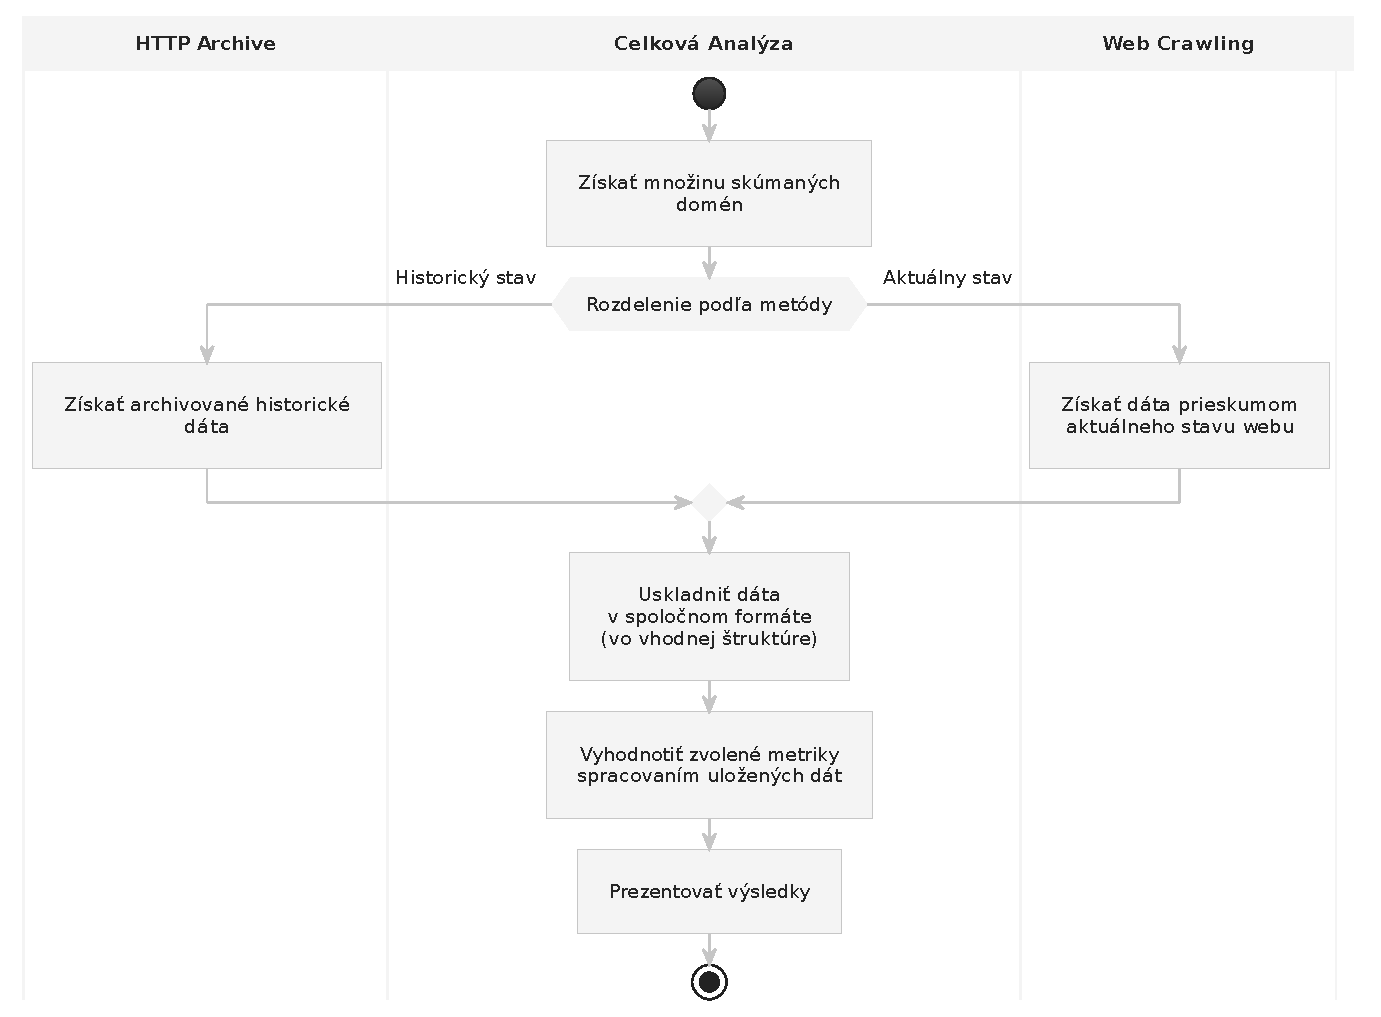
\includegraphics[scale=0.65]{obrazky-figures/analysis-activity-diagram-revised.pdf}    
 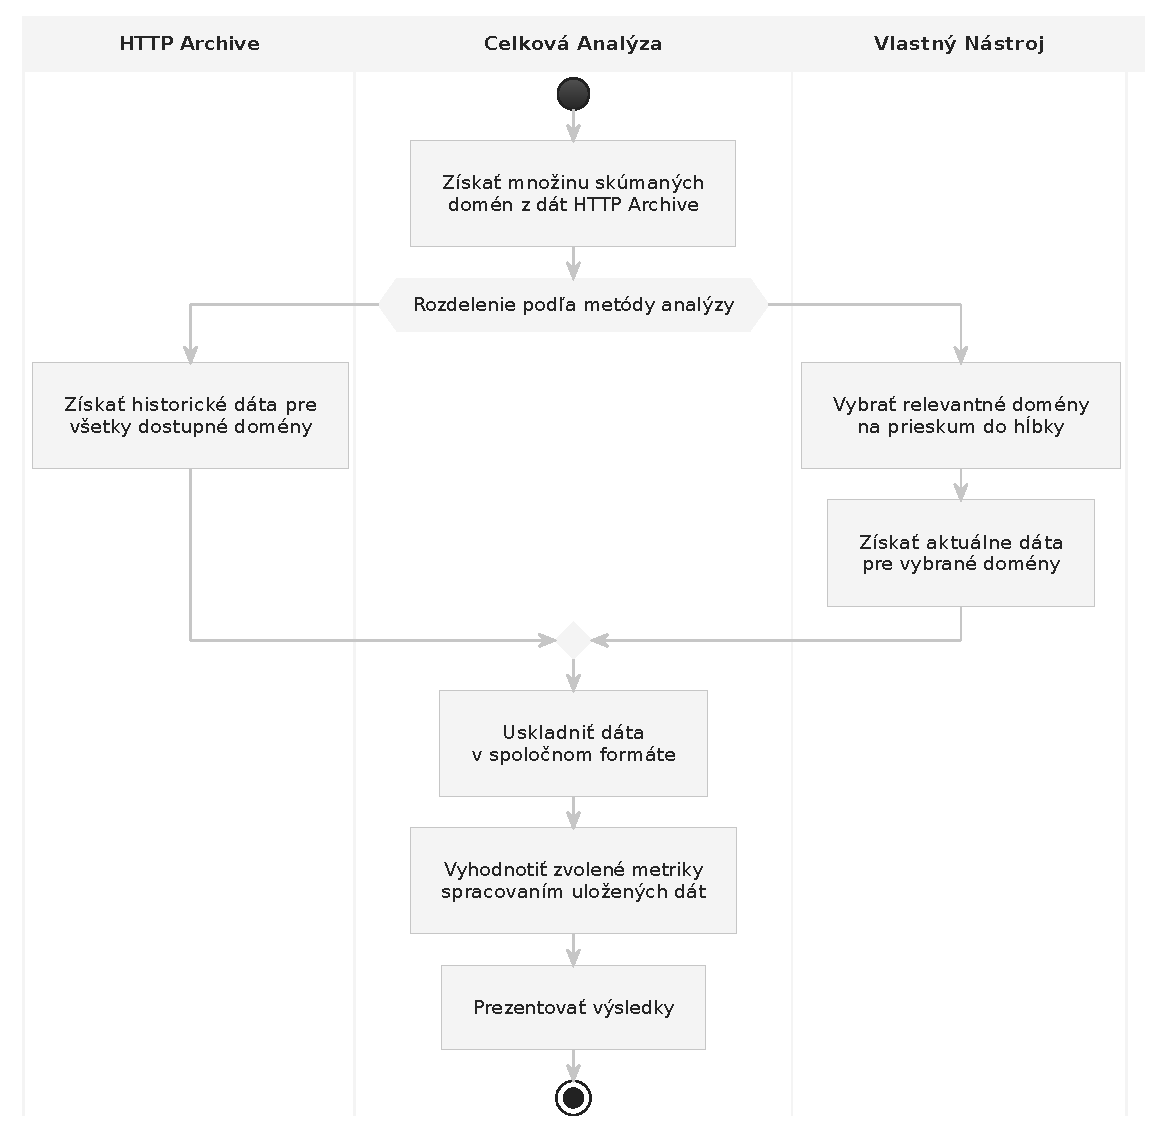
\includegraphics[scale=0.76]{obrazky-figures/analysis-activity-diagram-final.pdf}    
 \caption{Diagram aktivít analýzy.}
 \label{img:analysis-activity-diagram}
\end{center}
\end{figure}
